\documentclass{article}
\usepackage[utf8]{inputenc}
\usepackage{float}
\usepackage{xcolor}
\usepackage{graphicx}
\usepackage{amsmath}
\usepackage{amssymb}
\usepackage{placeins}
\usepackage{booktabs}
\usepackage{caption}
\usepackage{makecell}

\usepackage{hyperref}
\usepackage{textcomp}
\hypersetup{
    colorlinks=true,
    linkcolor=blue,
    filecolor=magenta,      
    urlcolor=blue,
}

\title{Scientific Computing - Molecular dynamics \\ Group F}
\newcommand{\subtitle}{Problem sheet 5}
\author{
    Jimin Kim \\
    Christian Nix \\
    Noah Schlenker
}
\date{\today}

\begin{document}

\maketitle

\begin{center}
    \LARGE \subtitle{}
\end{center}

\section{Pull request}
\label{sec:pr}
The pull request can be found \href{https://github.com/noahpy/MolSim-SS24/pull/60}{here}.

All new features have been tested with their according Unit tests (see \texttt{tests}) and have XML adaptations respectively.

\section{Membrane simulation}
\label{sec:mem}

    \subsection{Molecular abstraction}
    \label{sec:mem:mol}
        \begin{itemize}
            \item To allow future extensions of the code base with different molecules and their potentials (eg. rotation, ...) we abstracted a molecule class that calculates its own intra-molecular forces using the virtual \texttt{calculateIntraMolecularForces} method
            \item To allow for different structures, the molecule class offers a virtual \texttt{generateMolecule} method to construct the molecule into the container
        \end{itemize}

    \subsection{Membrane class}
    \label{sec:mem:mem}
        \begin{itemize}
            \item The membrane class inherits from the molecule class and overwrites the \texttt{calculateIntraMolecularForces} and \texttt{generateMolecule} methods
            \item Essentially, a membrane is generated exactly as a cuboid cluster would, except that we store maps of neighboring particles 
            \item We introduced a unique ID attribute for particles (which is their index within the particle cluster). This allowed us to store only the molecular IDs in the neighbor maps, which is both more memory-efficient and memory safe than storing reference wrappers
            \item We separated direct and diagonal neighbors into distinct maps for quick differentiation when calculating harmonic potentials.
            \item By storing only the top, top-right, right, and bottom-right neighbors (half of the neighbors) of a molecular particle, we enabled parallel force calculations by using Newton's third law (stencil idea which is also used in the parallelization of the force calculations later on).
            \item The neighbor relations within a membrane can be conceptualized as a directional non-cyclic graph with a single root (illustrated in Figure \ref{fig:mem}). Thus the force calculation can be done at any point in the graph at any time without calculating the forces twice.
            \item We added functions for the calculation of truncated intra-molecular and harmonic forces. The Lennard-Jones potential function was reused from the previous assignment while only applying it to non-neighbors that are close enough to repel each other ($dist = \sqrt[\leftroot{-2}\uproot{2}6]{2} \cdot \sigma$).
            \item The new simulation class, \texttt{MembraneSimulation}, extends \texttt{MixedLJSimulation} and manages the membrane initialization and generation accordingly. The rest of the simulation is the same
            \item The force calculation must also be adapted to not apply Lennard-Jones forces to particles within the membrane (we added a new function to include in the according strategy pattern)
        \end{itemize}

\begin{figure}[H]
    \centering
    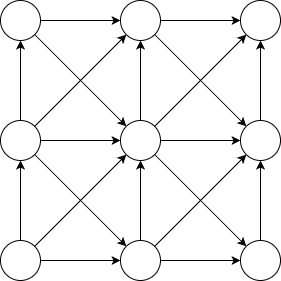
\includegraphics[width=0.3\textwidth]{../../res/membraneNeighbor.drawio}
    \caption{Illustration of neighbor relations in the membrane.}
    \label{fig:mem}
\end{figure}

\section{Parallelization}
\label{sec:para}

    \begin{itemize}
        \item The parallelization of our program primarily focused on iterating particles for calculations.
        \item A mutex was added to particles to prevent race conditions.
        \item We encountered issues with the parallelization of force calculations due to the handling of cell iteration, requiring significant adjustments to our cell grid.
        \item The runtime distribution can be seen here\ \ref{fig:runtime}.
    \end{itemize}

\begin{figure}[H]
    \centering
    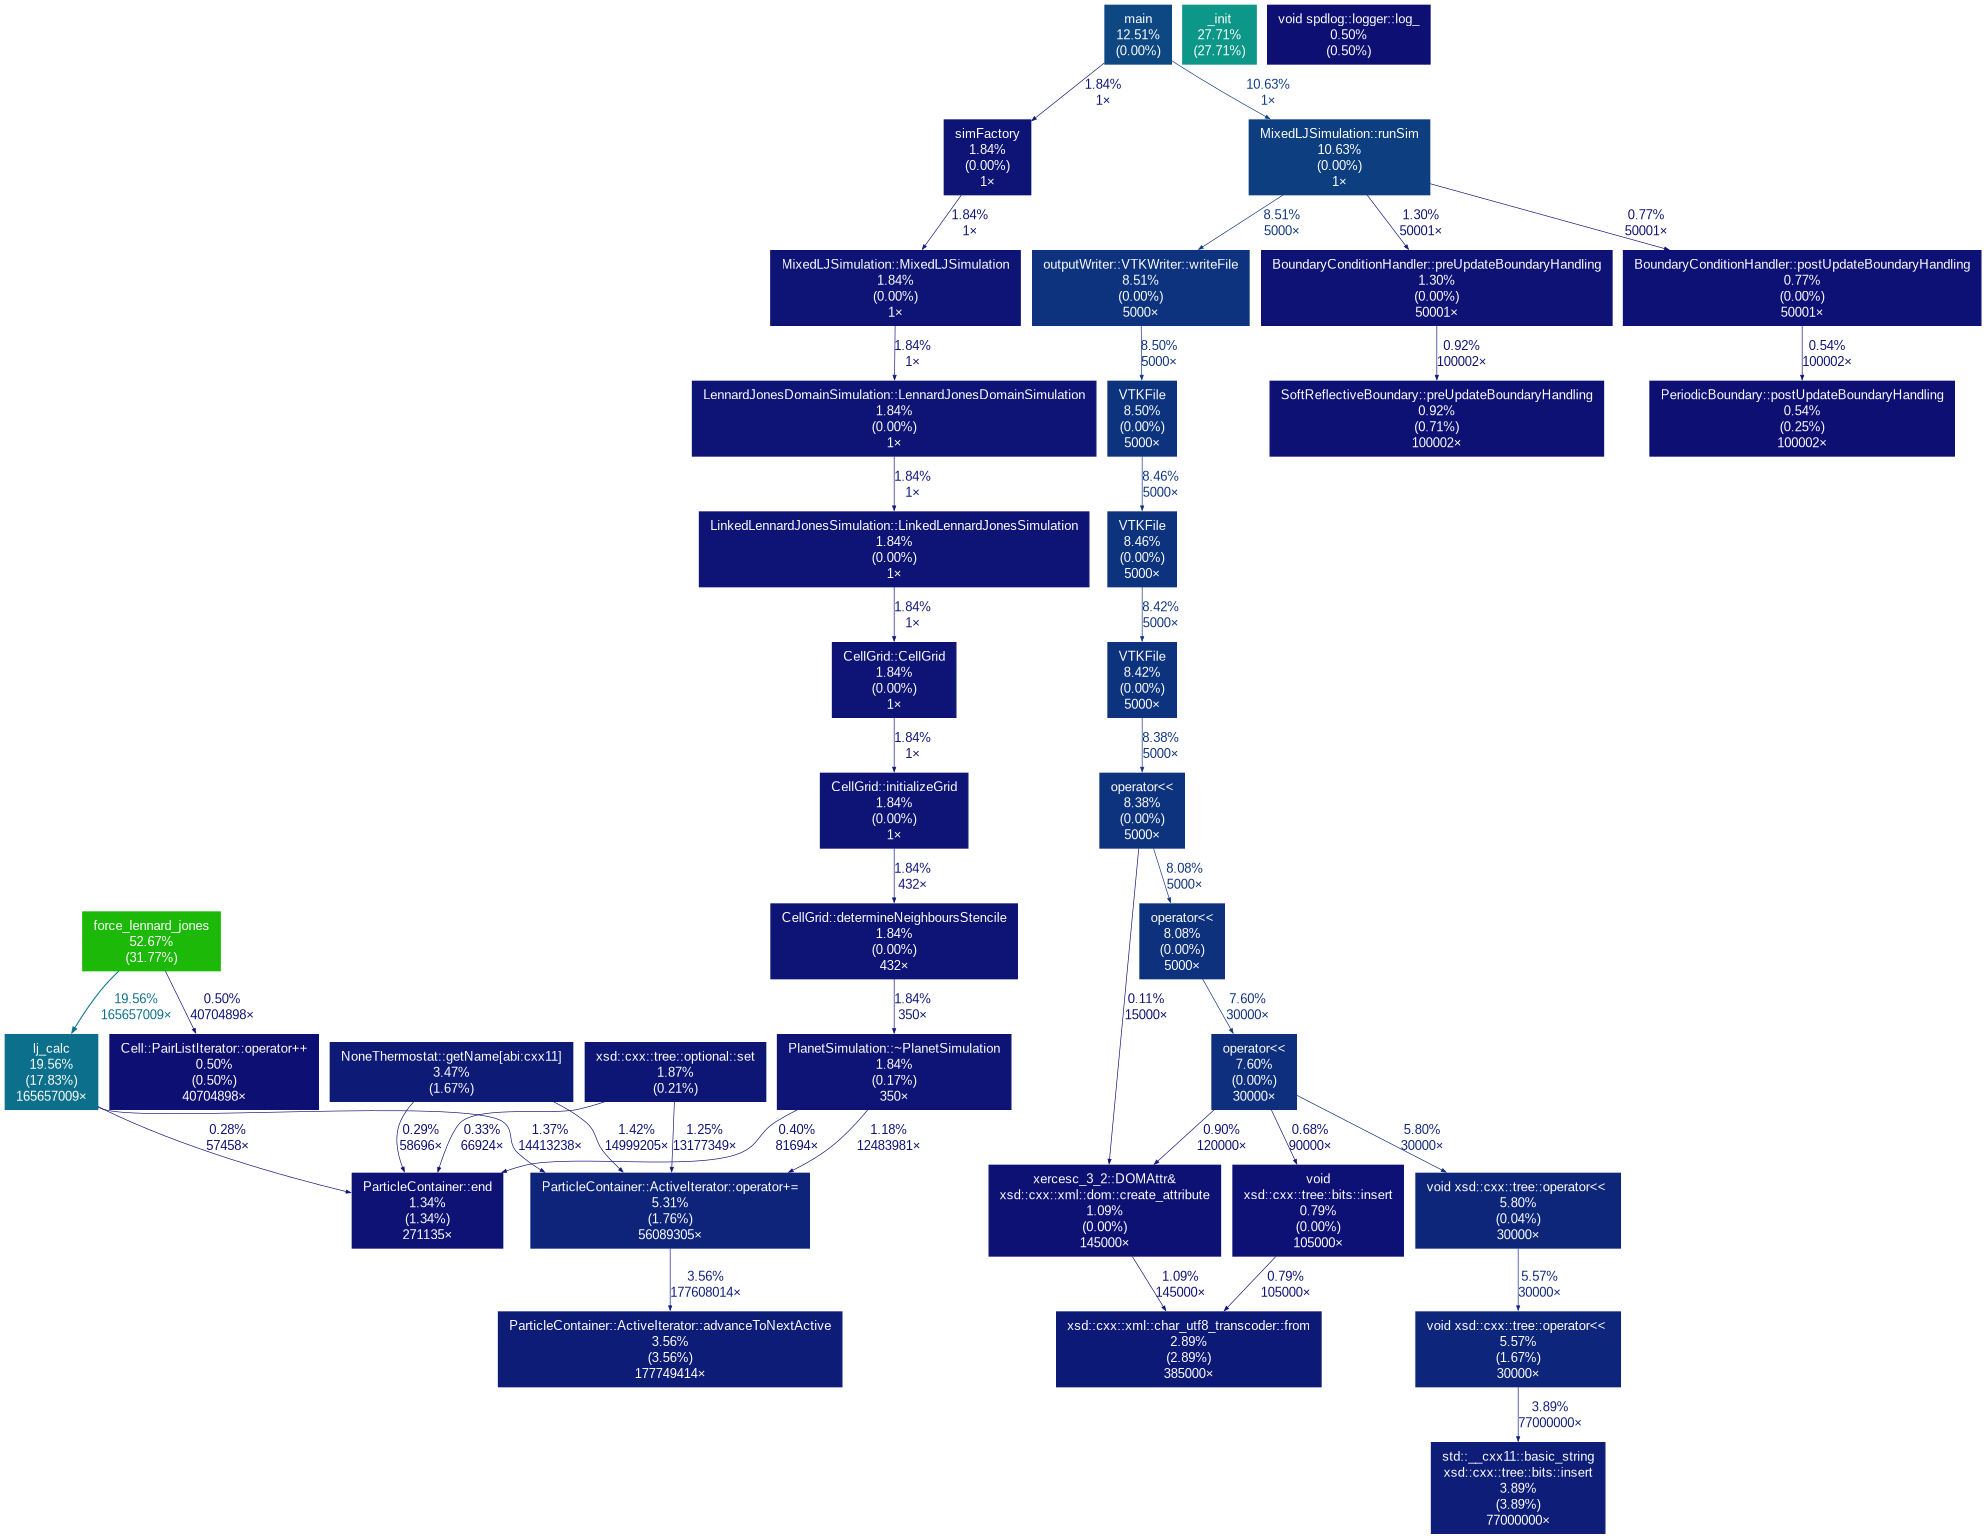
\includegraphics[width=1.3\textwidth]{../../res/runtimeVisualized}
    \caption{Visualization of runtime distributions.}
    \label{fig:runtime}
\end{figure}

\section{Nano-scale flow simulation}
\label{sec:nano}

The nano flow simulations did not require new physics and had most of the elements in place \textit{a priori}, which is why we decided to tackle option A.

\subsection{Experimental setups}
\label{sec:nano:exp}

    \begin{itemize}
        \item 
    \end{itemize}

\subsection{Videos}
\label{sec:nano:video}

    \begin{itemize}
        \item Here a list of all videos for the simulation.
        \item The simulation parameters were set to the specified values in the assignment sheet, if not stated otherwise.
        \begin{itemize}
            \item Standard simulation run: \href{https://youtu.be/-eWISjhgIgA}{here}
            \item Addition of small cluster of particles: \href{https://youtu.be/G34H3SCnpW0}{here}
            \item Lennard-Jones parameters of the walls set to $\sigma = 0.8$ and $\epsilon = 5.0$: \href{https://youtu.be/I4h6tjnJVuI}{here}
            \item Thermostat frequency set to 1000, gravity constant set to -9.81, and the Lennard-Jones parameters of the walls set to $\sigma = 0.8$ and $\epsilon = 5.0$: \href{https://youtu.be/yxNYmXJg5r0}{here}
        \end{itemize}
    \end{itemize}

\subsection{Implementation of the flow simulation}
\label{sec:nano:impl}

    \subsubsection{Immobilization}
    \label{sec:nano:impl:immob}
        \begin{itemize}
            \item To fix particles and make them immovable, we added a new input specification where particle types could be marked immobile.
            \item For that we had to introduce a new boolean attribute to particles to mark them as stationary.
            \item Within the velocity and positional calculations, we disregard any particles that are immobilized.
            \item Adjustments were made to the generation, boundary, and calculation files to accommodate stationary particles.
            \item The feature of immobile particles is backwards compatible so that even the base simulation has the option to have immobile particles.
        \end{itemize}

    \subsection{Thermostat}
    \label{sec:nano:impl:thermo}
        \begin{itemize}
            \item For the nano flow simulation a new thermostat class was implemented - \texttt{thermostat/IndividualThermostat}
            \item This thermostat will ignore fixed particles and perform temperature updates without changing the mean velocity of the particles.
            \item The selection of the thermostat is now decided via a factory function. The thermostat can be turned off by selecting the \texttt{NoneThermostat} or setting the frequency of thermal updates to 0.
            \item This approach allowed us to run the simulation without creating a new simulation class and by simply specifying simulation parameters.
        \end{itemize}


\subsection{Analytics}
\label{sec:nano:ana}

    \begin{itemize}
        \item We added a class \texttt{analytics/Analyzer} that can write density and velocity profiles to a .csv file for later analysis.
        \item The specification of analysis frequency and output file name can be done using the xml attributes.
        \item Also, it is possible to specify the number of bins to look at. This is even possible in multiple dimensions, allowing for more fine-grained analytics.
        \item As the .csv is only in 1D we needed to flatten the data using the following formula:
        \[
        \text{1D Index} = \text{x-Index} + \text{y-Index} \cdot \text{\#x-Bins} + \text{z-Index} \cdot \text{\#x-Bins} \cdot \text{\#y-Bins}
        \]
        \item The resulting profiles can then be plotted to a 2D heat map and 2D graph via a python script in \texttt{scripts/plots}.
        \item In our simulations we decided to have bins in 2 dimensions. The resulting heat map can be interpreted as the velocity / density profile of slices on top of the x-z-plane. The graph is simply the collapsed version onto the x-axis (see Figure \ref{fig:plot_xmpl}).
        \item In the videos of the nano flow simulations in Section \ref{sec:nano:video} the plotted diagrams for density and velocity can be seen next to the running simulation.
    \end{itemize}

    \begin{figure}[H]
        \centering
        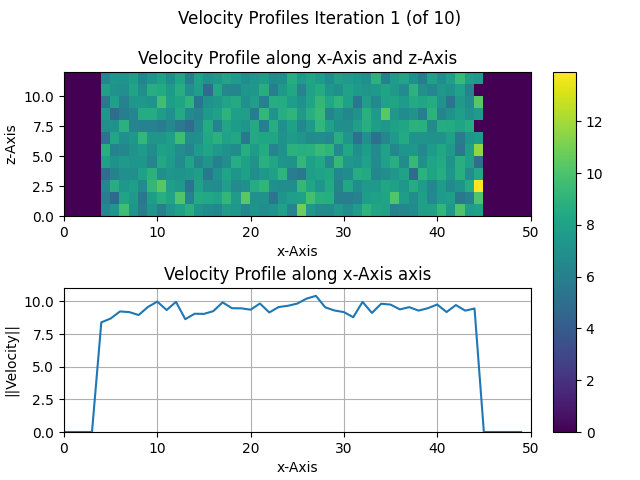
\includegraphics[width=1\textwidth]{../../res/Profile_example.png}
        \caption{Example of our profiling plots. The heat map is a visualization of velocities along the y-axis on top of the x-z plane. The graph is the collapsed versions onto the x-axis. }
        \label{fig:plot_xmpl}
    \end{figure}

    \begin{itemize}
        \item Regarding feedback from previous assignments and continuously increasing run-times, we added a progress logger to let the user know about the estimated time the simulation will still take to complete.
        \item This is also a nice quality of life feature as it is a simple sign that the simulation is progressing
    \end{itemize}

\end{document}
